\documentclass[10pt,twocolumn,letterpaper]{article}
\usepackage[utf8]{inputenc}
\usepackage[T1]{fontenc}
\usepackage{times}
\usepackage[letterpaper,top=0.75in,bottom=1in,left=0.65in,right=0.65in,columnsep=0.25in]{geometry}
\usepackage{graphicx,booktabs,tabularx,array,amsmath,cite,enumitem,microtype}
\usepackage[font=footnotesize,labelsep=period]{caption}
\usepackage{titlesec}
\usepackage[hidelinks]{hyperref}
\usepackage{listings}

% ---- Estilo IEEE (aproximacion sin IEEEtran) ----
\renewcommand{\thesection}{\Roman{section}}
\renewcommand{\thesubsection}{\Alph{subsection}}
\titleformat{\section}{\centering\normalsize\scshape}{\thesection.}{0.5em}{}
\titleformat{\subsection}{\normalsize\itshape}{\thesubsection.}{0.5em}{}
\titlespacing*{\section}{0pt}{8pt}{4pt}
\titlespacing*{\subsection}{0pt}{6pt}{3pt}
\renewcommand{\figurename}{Fig.}
\renewcommand{\tablename}{TABLA}
\renewcommand{\thetable}{\Roman{table}}
\captionsetup[table]{labelsep=newline,justification=centering,font={footnotesize,sc}}
\renewcommand{\refname}{Referencias}
\setlist{nosep,leftmargin=1.2em}
\lstset{basicstyle=\ttfamily\scriptsize,breaklines=true,frame=single,columns=fullflexible}
\setlength{\parskip}{0pt}

\title{\vspace{-1.2em}\LARGE Pluviómetro gravimétrico IoT con validación cruzada de sensores y despliegue serverless en AWS\\[0.3em]
\large Informe final del proyecto integrador}
\author{\normalsize Juan Sebastian Cruz Gallo\\
\small Facultad de Ingeniería de Datos e Inteligencia Artificial, Universidad Santo Tomás, Tunja, Colombia\\
\small Asignaturas: Cloud Computing · Sistemas de Adquisición y Procesamiento de Datos}
\date{\small Noviembre de 2026}

\begin{document}
\maketitle

\noindent\textbf{\textit{Abstract}---This report presents an IoT rain gauge that measures precipitation by weighing the collected water with a load cell (HX711, 24-bit) and validates the reading against a second physical principle: a float-driven potentiometer. An ESP32 applies a five-stage signal-processing chain (median filter, exponential smoothing, calibration, systematic-error correction and cross-validation with drift estimation) and publishes JSON telemetry over MQTT/TLS to AWS IoT Core. The prototype was built as a simulation: a digital twin models the raw sensor signals with white noise, drop impacts, wind, thermal drift, non-linearity, float friction and a 10~\% gain loss, and runs the same algorithm as the firmware, which was verified to produce identical quality flags (180/180 publications). In the twin, filtering reduced the mass RMSE from 4.33~g to 1.44~g; across 30 simulated storms there were no false alarms, the drift was always detected within 5~min, and the final rainfall error dropped from $-9.9$~\% to $-0.4$~\%. A serverless architecture (IoT rule, DynamoDB, Lambda, API Gateway, S3 and CloudFront), defined with Terraform, was deployed to an AWS account (29 resources, no errors) and validated end to end. The estimated cost is about USD 1 per month for one station. The project contributes to SDG 13 (Climate Action).}

\vspace{0.4em}
\noindent\textbf{\textit{Index Terms}---IoT, rain gauge, load cell, signal processing, digital twin, AWS IoT Core, serverless, Terraform, SDG 13.}

\section{Introducción}
La precipitación es una de las variables básicas de cualquier estación meteorológica y es determinante para la gestión del riesgo, la agricultura y el manejo del agua. Los pluviómetros de cubeta basculante, los más comunes en estaciones automáticas, pierden exactitud con lluvias intensas y no informan sobre la calidad del dato que entregan \cite{wmo8}.

Este proyecto propone un pluviómetro \emph{gravimétrico}: en lugar de contar descargas, pesa el agua recogida por un embudo de área conocida. Como 1~mm de lluvia equivale a 1~kg/m$^2$, la masa se convierte en milímetros de forma directa. Para que la señal sea confiable se mide la misma variable con un segundo principio físico (el nivel de agua mediante un flotador y un potenciómetro) y se comparan ambas lecturas. El dato procesado se envía a la nube de AWS, donde se almacena y se publica en un tablero web.

El prototipo se desarrolló como \emph{simulación}: no se construyó el montaje físico. En su lugar, un \emph{gemelo digital} reproduce la señal cruda de los sensores con sus fuentes de error y ejecuta el mismo algoritmo del firmware, lo que permite medir con números el efecto de cada etapa del tratamiento. El documento presenta el problema y su vínculo con un Objetivo de Desarrollo Sostenible (Sección~II), la estructura del sistema (Sección~III), el módulo de adquisición y procesamiento de datos con el gemelo digital (Sección~IV), el módulo de Cloud Computing (Sección~V) y las conclusiones, el alcance y las limitaciones (Sección~VI).

\section{Planteamiento del problema y vínculo con el ODS}
\subsection{Problema}
La información de lluvia a escala local suele ser escasa: las redes oficiales tienen estaciones distanciadas y los datos no siempre están disponibles en tiempo real. A esto se suma que un sensor de bajo costo, sin tratamiento de señal, entrega lecturas afectadas por ruido, deriva (\emph{drift}), sesgo y perturbaciones como el viento o el impacto de las gotas. Un dato de lluvia sin incertidumbre conocida puede llevar a decisiones equivocadas.

\noindent\textbf{Pregunta guía:} ¿cómo obtener datos de precipitación de bajo costo, en tiempo real y con una calidad cuantificada y visible para el usuario?

\subsection{Vínculo con el ODS 13: Acción por el clima}
El proyecto se alinea con el ODS~13 \cite{ods13}, en particular con la meta 13.1 (fortalecer la resiliencia y la capacidad de adaptación a los riesgos relacionados con el clima) y la meta 13.3 (mejorar la educación y la capacidad humana e institucional frente al cambio climático). Una red densa de pluviómetros económicos, con datos validados y publicados en línea, apoya la alerta temprana de lluvias intensas y la toma de decisiones locales. De forma secundaria aporta al ODS~6 (gestión del agua).

\subsection{Objetivos}
\textbf{General:} desarrollar un pluviómetro gravimétrico IoT con validación cruzada de sensores y un tablero desplegado en AWS mediante infraestructura como código.

\noindent\textbf{Específicos:} (1) diseñar la adquisición de una celda de carga y un potenciómetro con un ESP32 \cite{hx711,esp32}; (2) implementar un tratamiento de señal que cuantifique y corrija el error sistemático y la deriva; (3) validar el tratamiento con un gemelo digital de la señal; (4) desplegar una arquitectura serverless reproducible con Terraform; (5) estimar y optimizar el costo de operación en la nube.

\section{Estructura general del sistema}
El sistema se organiza en cuatro capas (Fig.~\ref{fig:arq}):
\begin{enumerate}
\item \textbf{Sensado:} celda de carga YZC-133 con módulo HX711 (principal) y potenciómetro lineal de 20~k$\Omega$ con flotador (redundante). En este proyecto se modelan en el gemelo digital y se simulan en Wokwi.
\item \textbf{Procesamiento en el borde:} el ESP32 filtra, calibra, corrige y valida la señal antes de enviarla, y adjunta una bandera de calidad a cada lectura.
\item \textbf{Nube:} AWS IoT Core recibe los mensajes MQTT; una regla los guarda en DynamoDB; una función Lambda los expone mediante API Gateway.
\item \textbf{Presentación:} un tablero HTML con Chart.js, alojado en S3 y distribuido con CloudFront, muestra lluvia acumulada, tasa, señal cruda frente a filtrada, comparación entre sensores y calidad.
\end{enumerate}

\begin{figure*}[t]
\centering
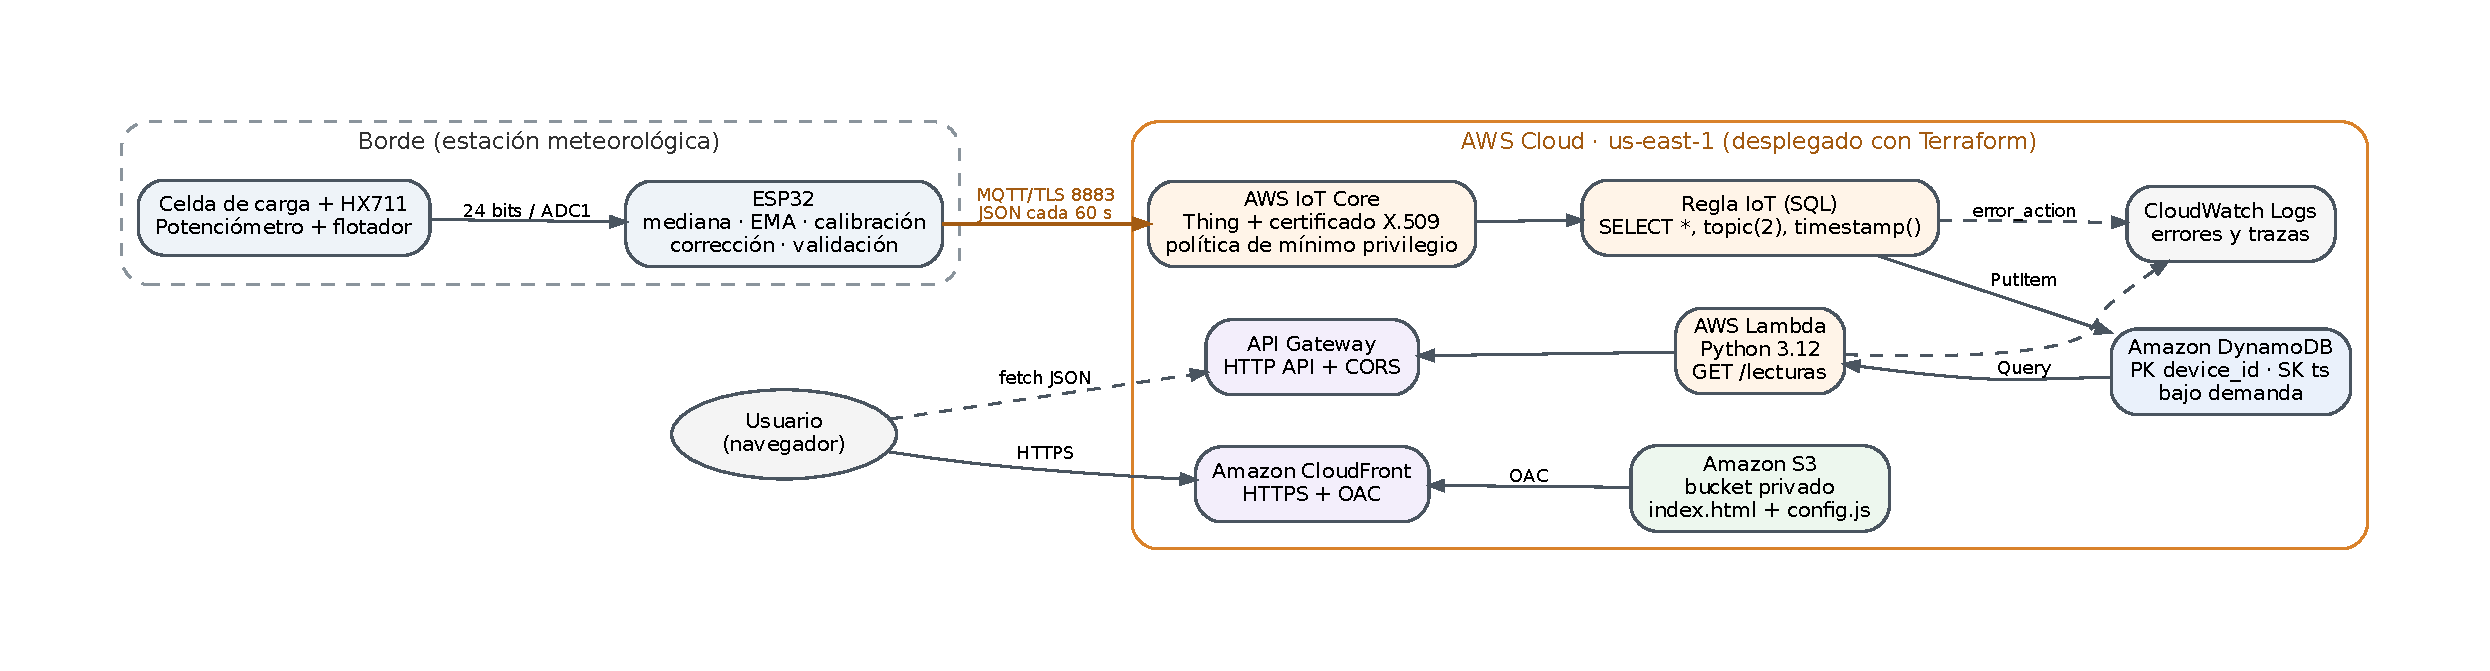
\includegraphics[width=0.96\textwidth]{../docs/arquitectura.pdf}
\caption{Arquitectura del sistema. Todos los recursos dentro del recuadro de AWS se crean con Terraform (\texttt{infra/terraform}).}
\label{fig:arq}
\end{figure*}

\section{Módulo de adquisición y procesamiento de datos}
\subsection{Principio de medición}
El embudo de 160~mm de diámetro tiene un área $A=\pi(0{,}08)^2\approx0{,}0201$~m$^2$. La lámina de lluvia se obtiene como
\begin{equation}
h\,[\text{mm}] = \frac{m\,[\text{kg}]}{A\,[\text{m}^2]}, \qquad 1~\text{mm}\approx 20{,}1~\text{g}.
\end{equation}
La capacidad útil del recipiente (2~kg) corresponde a unos 100~mm de lluvia, por lo que se recomienda una celda de 5~kg para ganar resolución.

\begin{table}[t]
\caption{Sensores del diseño}
\label{tab:sens}
\centering\footnotesize
\begin{tabularx}{\columnwidth}{@{}lXX@{}}
\toprule
 & Celda + HX711 & Potenciómetro 20 k$\Omega$\\
\midrule
Principio & Galgas en puente de Wheatstone & Divisor de tensión con flotador\\
Magnitud & Masa de agua & Nivel de agua\\
Interfaz & Serie (DT: GPIO16, SCK: GPIO4), 24 bits, ganancia 128 & ADC1 (GPIO34), 12 bits, \texttt{analogReadMilliVolts()}\\
Rol & Principal & Validación cruzada\\
\bottomrule
\end{tabularx}
\end{table}

\subsection{Tratamiento de la señal}
Cada muestra del HX711 (unas 10 por segundo) pasa por cinco etapas:
\begin{enumerate}
\item \textbf{Mediana de 5 muestras:} elimina picos por el impacto de las gotas.
\item \textbf{Media exponencial (EMA):} $y_k=\alpha x_k+(1-\alpha)y_{k-1}$, con $\alpha=0{,}15$.
\item \textbf{Calibración:} $m=(\text{raw}-\text{offset})/\text{factor}$, con la tara del recipiente vacío y el factor obtenido por regresión.
\item \textbf{Corrección del error sistemático:} a partir de la regresión $m_{\text{med}}=a\,m_{\text{real}}+b$ se corrige $x=(m_{\text{med}}-b)/a$; $b$ es el offset y $a\neq1$ el error de ganancia.
\item \textbf{Validación:} se marcan como \texttt{FUERA\_RANGO} las lecturas físicamente imposibles (lluvia negativa, saltos mayores a 200~g por intervalo, golpes o vaciado del recipiente) y en ese caso se publica el último valor válido. Las dos lecturas se comparan cuando hay más de 1~mm: están en desacuerdo si
\begin{equation}
|h_{\text{celda}}-h_{\text{pot}}| > \max(0{,}08\,h_{\text{pot}},\;0{,}8~\text{mm}).
\end{equation}
La parte relativa (8~\%) es menor que la deriva que se quiere detectar (10~\%); el piso absoluto de 0,8~mm cubre la resolución del flotador y se eligió con el gemelo digital (Sección~IV-D). Si el desacuerdo persiste durante 5 envíos seguidos, la ganancia de la celda se estima como la mediana de los últimos cinco cocientes y se compensa; la lectura se marca \texttt{SOSPECHOSA} mientras no está compensada y \texttt{CORREGIDA} cuando la compensación la devuelve a la banda.
\end{enumerate}

\subsection{Calibración y estimación del error}
El procedimiento de calibración consiste en verter cantidades conocidas de agua (0 a 2000~g), lo que calibra ambos sensores a la vez: tara con el recipiente vacío, un factor provisional con una masa de 1000~g y una regresión $m_{\text{med}}=a\,m_{\text{real}}+b$ sobre todos los puntos. El script \texttt{calibracion.py} y el gemelo digital aplican este método; en el gemelo, la celda tiene una no linealidad de 0,3~\% a plena carga. La regresión dio $a=1{,}0013$ y $b=-0{,}68$~g y redujo el RMSE de 1,04~g a 0,55~g (0,027~mm); el error residual es la curvatura que una recta no puede corregir (Fig.~\ref{fig:cal}). La recta del potenciómetro tuvo un RMSE de 0,15~mm.

\begin{figure}[t]
\centering
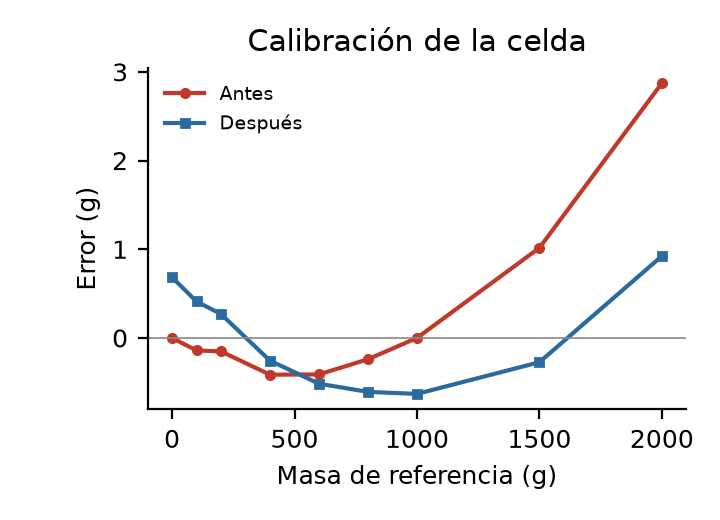
\includegraphics[width=0.85\columnwidth]{../simulacion/resultados/fig_calibracion.png}
\caption{Calibración de la celda en el gemelo digital: error antes y después de la corrección por regresión.}
\label{fig:cal}
\end{figure}

\subsection{Gemelo digital de la señal}
Como no se construyó el montaje físico, el tratamiento se validó con un gemelo digital (\texttt{simulacion/gemelo\_digital.py}). Simula una tormenta de 3~h con tres chubascos (hasta 30~mm/h, 32,7~mm en total), genera la señal cruda que entregarían el HX711 a 10 muestras/s y el potenciómetro, y le aplica el mismo tratamiento del firmware. La Tabla~\ref{tab:fuentes} resume las fuentes de error modeladas.

\begin{table}[t]
\caption{Fuentes de error del gemelo digital}
\label{tab:fuentes}
\centering\footnotesize
\begin{tabularx}{\columnwidth}{@{}lX@{}}
\toprule
Fuente & Modelo\\
\midrule
Ruido del HX711 & Gaussiano, $\sigma=0{,}25$~g por muestra\\
Impacto de gotas & Poisson proporcional a la intensidad, impulsos de 15~g en promedio\\
Viento & Ruido de baja frecuencia AR(1), hasta 1,5~g\\
Deriva térmica & Offset senoidal de $\pm1{,}2$~g\\
No linealidad & $+1{,}5\times10^{-6}\,m^2$ (0,3~\% a 2~kg)\\
Golpe al equipo & +400~g durante 90~s a las 0,95~h\\
Falla de ganancia & Caída al 90~\% con rampa de 5~min desde las 2,2~h\\
Potenciómetro & Ruido de 8~mV, promedio de 16 lecturas, no linealidad de 15~mV y zona muerta de 0,3~mm por fricción\\
\bottomrule
\end{tabularx}
\end{table}

\textbf{Filtros.} La Tabla~\ref{tab:filtros} compara la masa en cada etapa frente a la masa real durante la lluvia. La mediana elimina los impactos (error máximo de 104~g a 24~g) y la EMA suaviza el resto (8,4~g); su constante de tiempo es de 0,57~s, despreciable frente al envío cada 60~s (Fig.~\ref{fig:filtros}).

\begin{table}[t]
\caption{Error de la masa frente a la real, con lluvia}
\label{tab:filtros}
\centering\footnotesize
\begin{tabular}{@{}lrr@{}}
\toprule
Etapa & RMSE (g) & Error máx. (g)\\
\midrule
Señal cruda & 4,33 & 104,4\\
Mediana de 5 & 1,51 & 23,8\\
Mediana + EMA & 1,44 & 8,4\\
\bottomrule
\end{tabular}
\end{table}

\begin{figure}[t]
\centering
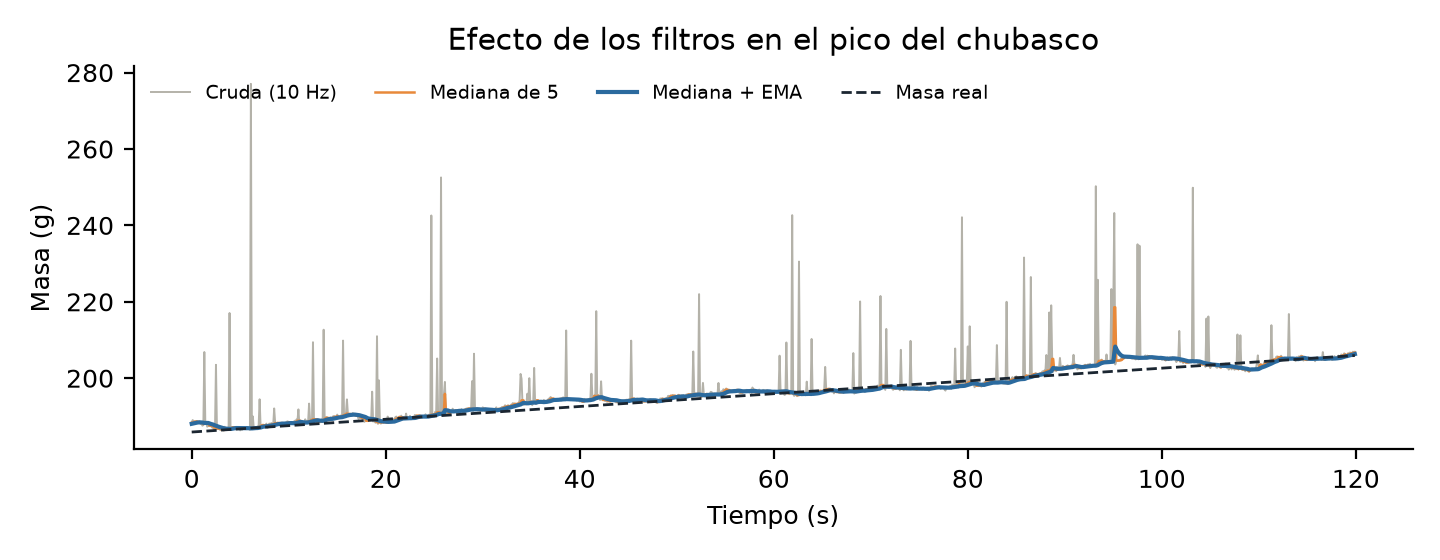
\includegraphics[width=\columnwidth]{../simulacion/resultados/fig_filtros.png}
\caption{Dos minutos de señal en el pico del primer chubasco: la mediana elimina los picos por impacto de gotas y la EMA suaviza el ruido restante.}
\label{fig:filtros}
\end{figure}

\textbf{Regla de validación.} La primera versión usaba solo el cociente con tolerancia de $\pm8$~\%. El gemelo mostró que con poca lluvia acumulada genera falsas alarmas: cuando el nivel sube rápido, la fricción del flotador atrasa al potenciómetro unos 0,3~mm, que con 3--6~mm acumulados ya es un 10~\%. La Fig.~\ref{fig:umbral} compara reglas: subir el mínimo a 5~mm reduce las falsas alarmas al 0,8~\% pero deja sin validar los primeros milímetros; agregar un piso absoluto de 0,8~mm las elimina sin retrasar la detección de la deriva. Esa es la regla adoptada en el firmware.

\begin{figure}[t]
\centering
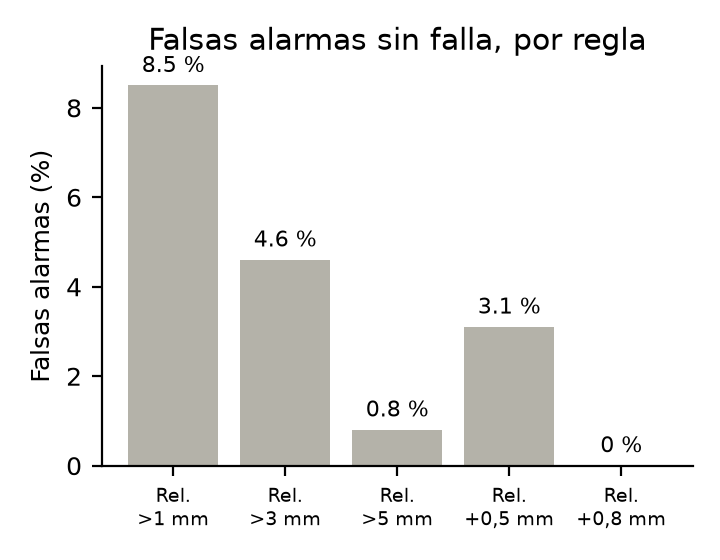
\includegraphics[width=0.8\columnwidth]{../simulacion/resultados/fig_umbral.png}
\caption{Porcentaje de lecturas marcadas sin que exista falla, antes de la deriva, según la regla de validación.}
\label{fig:umbral}
\end{figure}

\subsection{Detección y corrección de la deriva}
La Fig.~\ref{fig:val} muestra la tormenta completa. El golpe de 90~s se marcó \texttt{FUERA\_RANGO} y no alteró la lluvia publicada. Al iniciar la falla de ganancia, la lectura sin compensar se separa del potenciómetro; a los 5~min, cuando la pérdida de ganancia supera el 8~\%, las lecturas pasan a \texttt{SOSPECHOSA}, y a los 9~min la ganancia estimada (0,905 frente a 0,90 real) ya se compensa y las lecturas quedan \texttt{CORREGIDA}. La tasa de lluvia se calcula con la misma ganancia en los dos envíos, para que la activación de la compensación no se interprete como lluvia. Al final de la tormenta la lluvia sin compensar tenía un error de $-9{,}9$~\% y la corregida de $-0{,}4$~\%.

\begin{figure*}[t]
\centering
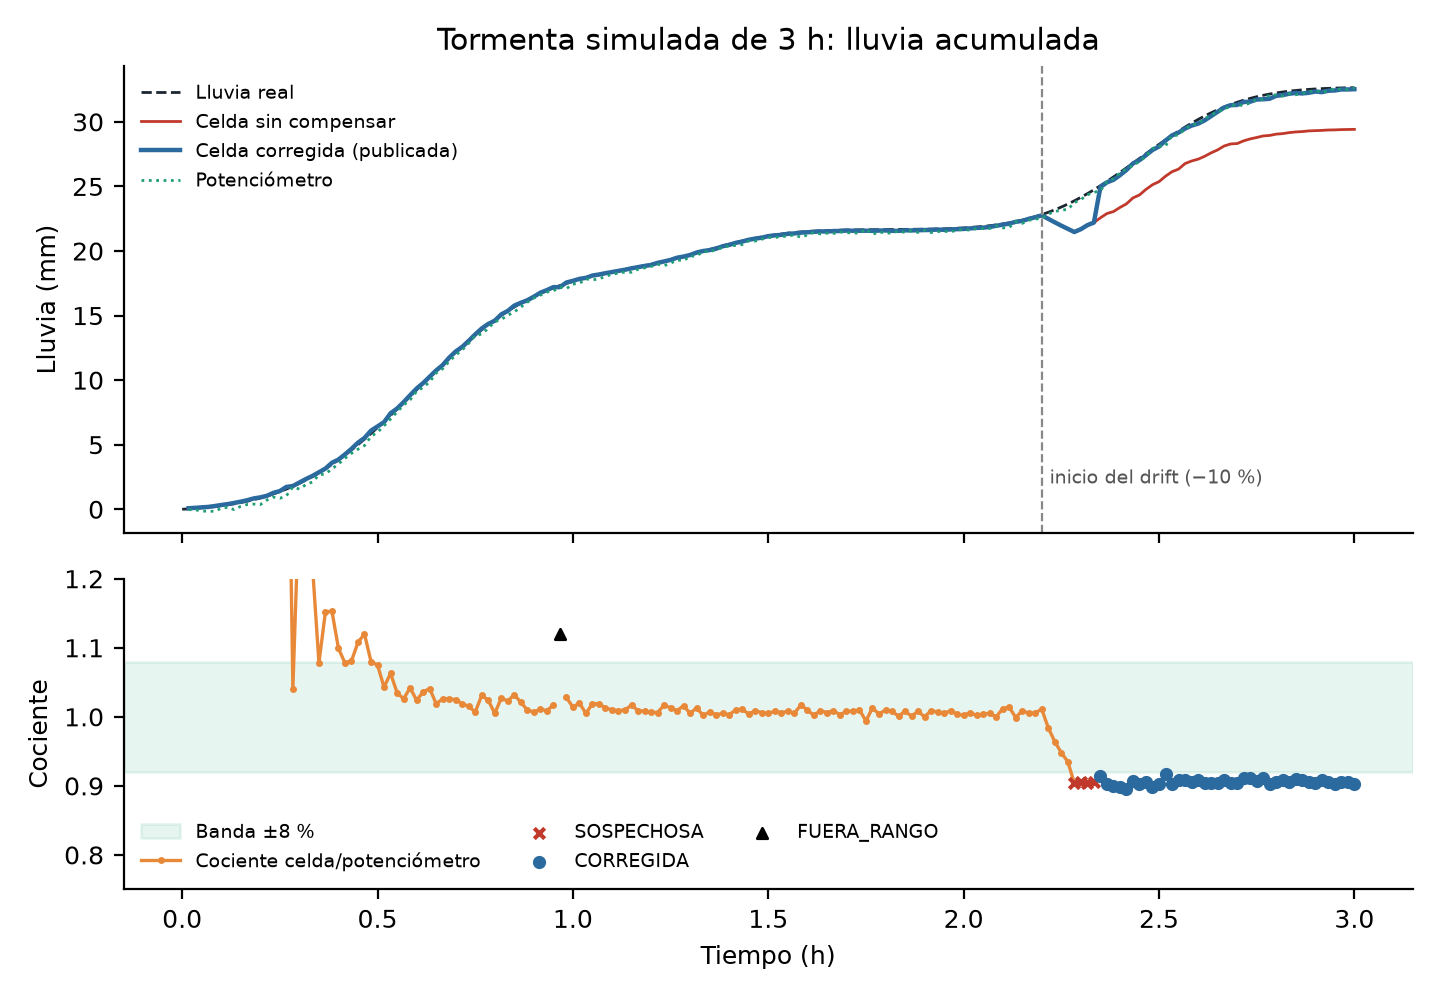
\includegraphics[width=0.78\textwidth]{../simulacion/resultados/fig_validacion.png}
\caption{Tormenta simulada de 3~h. Arriba: lluvia real, lectura de la celda sin compensar, lectura corregida que publica el sistema y potenciómetro. Abajo: cociente celda/potenciómetro, banda de $\pm8$~\% y bandera de calidad de cada envío.}
\label{fig:val}
\end{figure*}

Para comprobar que el resultado no depende de una realización del ruido, la tormenta se repitió con 30 semillas distintas (Tabla~\ref{tab:mc}).

\begin{table}[t]
\caption{Robustez en 30 tormentas simuladas}
\label{tab:mc}
\centering\footnotesize
\begin{tabular}{@{}lr@{}}
\toprule
Métrica & Resultado\\
\midrule
Falsas alarmas antes de la deriva & 0~\% (máx. 0~\%)\\
Deriva detectada & 100~\%\\
Tiempo de detección & 5,0~min\\
Error final sin compensar (media) & $-9{,}89$~\%\\
Error final corregido (media) & $-0{,}41$~\%\\
Error final corregido (máx. absoluto) & 0,61~\%\\
Golpe detectado & 100~\%\\
\bottomrule
\end{tabular}
\end{table}

\subsection{Equivalencia entre firmware y gemelo}
Para asegurar que lo validado es lo que ejecutaría el ESP32, el firmware se compiló en el computador con \texttt{g++}, reemplazando las librerías de Arduino por \emph{stubs}: el HX711 entrega la señal cruda del gemelo y el reloj avanza 100~ms por muestra (\texttt{simulacion/prueba\_firmware}). Las 180 publicaciones del firmware tuvieron la misma bandera de calidad que las del gemelo (135 \texttt{OK}, 4 \texttt{SOSPECHOSA}, 40 \texttt{CORREGIDA}, 1 \texttt{FUERA\_RANGO}); la lluvia publicada difirió como máximo 0,15~mm, por el ruido del potenciómetro que solo añade el gemelo.

\section{Módulo de Cloud Computing}
\subsection{Arquitectura seleccionada}
Se eligió una arquitectura \emph{serverless} administrada en la región \texttt{us-east-1}. Las razones son: (1) el costo es proporcional al uso y casi nulo para un prototipo; (2) no hay servidores que administrar ni parchar; (3) los servicios escalan sin cambios de diseño a una red de estaciones; y (4) todos están disponibles en AWS Academy Learner Lab. La Tabla~\ref{tab:serv} resume cada componente.

\begin{table}[t]
\caption{Servicios de AWS y función en el sistema}
\label{tab:serv}
\centering\footnotesize
\begin{tabularx}{\columnwidth}{@{}lX@{}}
\toprule
Servicio & Función\\
\midrule
IoT Core & Broker MQTT/TLS; \emph{Thing}, certificado X.509 y política que solo permite conectarse con su ID y publicar en \texttt{pluviometro/<id>/*}.\\
Regla IoT & \texttt{SELECT *, topic(2) AS device\_id, timestamp() AS ts}; escribe en DynamoDB y registra errores en CloudWatch.\\
DynamoDB & Serie de tiempo; clave de partición \texttt{device\_id}, de orden \texttt{ts}; modo bajo demanda.\\
Lambda & Python 3.12; \texttt{GET /lecturas} con parámetros \texttt{horas} y \texttt{desde} (consulta incremental).\\
API Gateway & HTTP API con CORS y límite de 10 solicitudes/s.\\
S3 + CloudFront & Tablero estático; bucket privado leído solo por CloudFront mediante OAC; HTTPS.\\
CloudWatch & Logs de la Lambda y de errores de la regla (retención de 7 días).\\
\bottomrule
\end{tabularx}
\end{table}

\subsection{Infraestructura como código (Terraform)}
Toda la infraestructura se declara con Terraform \cite{tf} en \texttt{infra/terraform}, organizada por responsabilidad: \texttt{iot.tf}, \texttt{data.tf}, \texttt{api.tf}, \texttt{frontend.tf}, \texttt{iam.tf}, \texttt{firmware\_secrets.tf}, variables y salidas. Aspectos de diseño:
\begin{itemize}
\item \textbf{Compatibilidad con AWS Academy:} el Learner Lab no permite crear roles IAM; con \texttt{use\_lab\_role = true} se reutiliza \texttt{LabRole}, y con \texttt{false} se crean roles de mínimo privilegio para una cuenta propia.
\item \textbf{Sin valores fijos:} Terraform genera \texttt{config.js} con la URL real de la API y el archivo \texttt{aws\_secrets.h} del firmware con el endpoint, el certificado y la llave privada, que se excluye del repositorio mediante \texttt{.gitignore}.
\item \textbf{Seguridad:} TLS 1.2 con certificados X.509, política IoT restringida, bucket sin acceso público y limitación de solicitudes en la API.
\end{itemize}
El despliegue completo se reproduce con:
\begin{lstlisting}
cd infra/terraform
cp terraform.tfvars.example terraform.tfvars
terraform init
terraform plan
terraform apply
terraform output   # endpoint MQTT, URL de la API y del tablero
\end{lstlisting}
y se elimina con \texttt{terraform destroy} al terminar cada sesión del laboratorio para no consumir créditos.

\begin{figure*}[t]
\centering
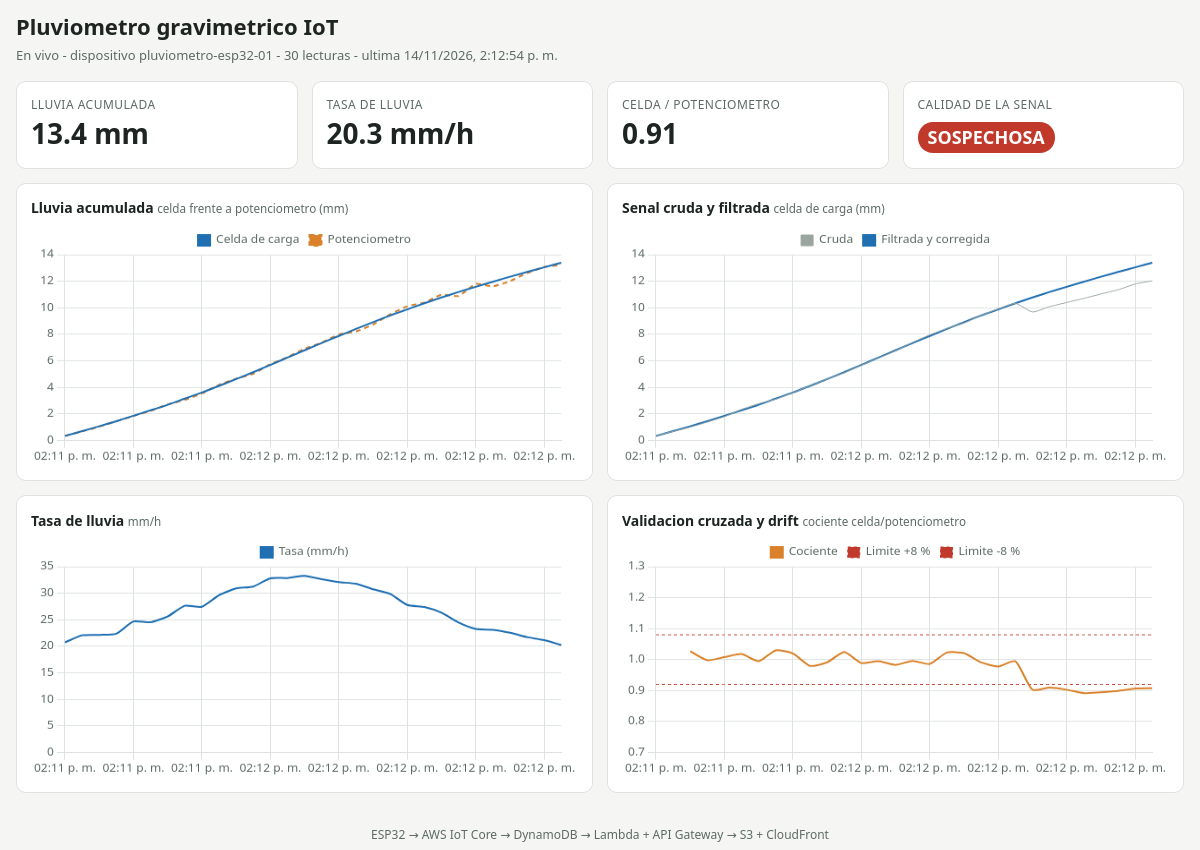
\includegraphics[width=0.78\textwidth]{../docs/evidencia/dashboard_informe.png}
\caption{Tablero en CloudFront con las 30 lecturas de la prueba. En el panel de validación cruzada, el cociente sale de la banda $\pm8$~\% al activarse la deriva simulada, mientras la lluvia filtrada y corregida continúa sin caída.}
\label{fig:dash}
\end{figure*}

\subsection{Estimación preliminar de costos}
Los valores de la Tabla~\ref{tab:cost} los calcula el script de costos del repositorio (carpeta \texttt{costos}) con precios de lista de la región \texttt{us-east-1}, sin capa gratuita (escenario conservador) \cite{awsiot,awsddb,awsapigw}. Con la capa gratuita de 12 meses, el prototipo tendría costo prácticamente nulo.

\begin{table}[t]
\caption{Costo mensual estimado (USD)}
\label{tab:cost}
\centering\footnotesize
\begin{tabular}{@{}lrrrr@{}}
\toprule
Concepto & Prot. & Demo & Demo opt. & Red opt.\\
\midrule
IoT Core & 0,06 & 0,34 & 0,34 & 2,98\\
DynamoDB escritura & 0,03 & 0,16 & 0,16 & 1,35\\
DynamoDB lectura & 0,67 & 13,30 & 0,13 & 0,55\\
DynamoDB almac. & 0,00 & 0,02 & 0,02 & 0,19\\
Lambda + API GW & 0,16 & 0,53 & 0,53 & 7,95\\
S3, CloudFront, logs & 0,02 & 0,06 & 0,06 & 0,76\\
\midrule
\textbf{Total} & \textbf{0,94} & \textbf{14,42} & \textbf{1,25} & \textbf{13,77}\\
\bottomrule
\end{tabular}
\vspace{0.2em}

\raggedright\scriptsize Prot.: 1 estación, 1 msg/min, 3 usuarios 8 h/día. Demo: 1 msg/10 s, 10 usuarios. Red: 50 estaciones, 50 usuarios 24 h/día. ``Opt.'': el tablero solo pide lecturas nuevas.
\end{table}

El análisis mostró que el costo dominante no era la ingesta sino las \emph{lecturas} de DynamoDB, porque el tablero volvía a descargar 24~h de datos cada 30~s. Con la consulta incremental (parámetro \texttt{desde}) el costo del escenario de demostración baja de 14,42 a 1,25~USD/mes (91~\%). Esta optimización ya está implementada en la Lambda y en el tablero.

\subsection{Evidencia de ejecución}\label{sec:evid}
La infraestructura se desplegó en una cuenta propia de AWS (\texttt{us-east-1}) con \texttt{use\_lab\_role = false}, de modo que Terraform creó los dos roles IAM de mínimo privilegio (escritura en DynamoDB para la regla IoT; consulta de la tabla y logs para la Lambda). \texttt{terraform apply} creó los 29 recursos del plan sin errores. Después, al ajustar la tolerancia de validación del tablero, \texttt{terraform plan} detectó solo el cambio de \texttt{index.html} y el \texttt{apply} modificó un único recurso (0 creados, 1 cambiado, 0 destruidos), lo que ilustra el cambio incremental con IaC. Las salidas se resumen en la Tabla~\ref{tab:out}; el número de cuenta se omite en las evidencias de texto.

\begin{table}[t]
\caption{Salidas de \texttt{terraform output}}
\label{tab:out}
\centering\scriptsize
\begin{tabularx}{\columnwidth}{@{}l>{\raggedright\arraybackslash\ttfamily}X@{}}
\toprule
Salida & Valor\\
\midrule
\texttt{iot\_endpoint} & ao0jmtgzs4irm-ats.\allowbreak iot.us-east-1.amazonaws.com\\
\texttt{mqtt\_topic} & pluviometro/\allowbreak pluviometro-esp32-01/\allowbreak telemetria\\
\texttt{dynamodb\_table} & pluviometro-lecturas\\
\texttt{api\_url} & https://elsnkxxeb3.execute-api.us-east-1.\allowbreak amazonaws.com/lecturas\\
\texttt{dashboard\_url} & https://d2nb5zllocqacr.cloudfront.net\\
\texttt{certificate\_id} & a2712eddaf10\ldots 2b297a72b5d07 (ACTIVE)\\
\bottomrule
\end{tabularx}
\end{table}

La prueba de punta a punta, previa al gemelo digital, reprodujo la ruta completa del dato: se publicaron 30 mensajes MQTT con el formato del firmware en el tópico \texttt{pluviometro/\allowbreak pluviometro-esp32-01/\allowbreak telemetria} (\texttt{aws iot-data publish}); la regla IoT añadió \texttt{device\_id} y \texttt{ts} y los guardó en DynamoDB; la Lambda los entregó por API Gateway (\texttt{GET /lecturas}, HTTP 200, $n=30$), y el tablero servido por CloudFront los graficó (Fig.~\ref{fig:dash}). Se simuló una lluvia fuerte de 13,4~mm con intensidad entre 20 y 33~mm/h. En los mensajes 23 a 30 se activó la deriva simulada: la lectura cruda cayó al 90~\%, el cociente sin compensar quedó entre 0,89 y 0,91, por debajo del límite de 0,92, y las lecturas se marcaron \texttt{SOSPECHOSA}, mientras la lluvia corregida siguió la curva real sin caída (Tabla~\ref{tab:lect}). Antes de la deriva el cociente estuvo entre 0,98 y 1,03 y todas las lecturas fueron \texttt{OK}.

Fue una prueba acelerada: cada mensaje representa 1~minuto de lluvia simulada, pero se publicaron cada 2~s, por lo que el eje de tiempo del tablero abarca 1~minuto real. Las capturas de la consola de DynamoDB e IoT Core se incluyen en el Anexo~A. El 22 de noviembre de 2026 se publicaron en AWS IoT Core, en el mismo tópico, las 180 lecturas del gemelo digital (\texttt{-{}-publicar}): la API las devolvió completas y en orden, con sus banderas de calidad (135 \texttt{OK}, 1 \texttt{FUERA\_RANGO}, 4 \texttt{SOSPECHOSA} y 40 \texttt{CORREGIDA}). El tablero graficó las 180 y mostró la bandera de la última, \texttt{CORREGIDA}; la captura está en \texttt{docs/\allowbreak evidencia/\allowbreak dashboard\_gemelo.png}.

\begin{table}[t]
\caption{Lecturas almacenadas en DynamoDB}
\label{tab:lect}
\centering\footnotesize
\begin{tabular}{@{}rrrrl@{}}
\toprule
\texttt{seq} & \texttt{lluvia\_mm} & \texttt{lluvia\_pot\_mm} & \texttt{ratio} & \texttt{calidad}\\
\midrule
10 & 4,12 & 4,20 & 0,980 & OK\\
20 & 9,42 & 9,51 & 0,991 & OK\\
22 & 10,34 & 10,40 & 0,995 & OK\\
23 & 10,78 & 10,99 & 0,903 & SOSPECHOSA\\
30 & 13,39 & 13,21 & 0,908 & SOSPECHOSA\\
\bottomrule
\end{tabular}
\end{table}


\section{Conclusiones, alcance y limitaciones}
\subsection{Conclusiones}
\begin{itemize}
\item La cadena mediana + EMA reduce el error de la masa de 4,33~g a 1,44~g (RMSE) y el error máximo de 104~g a 8,4~g, con un retardo despreciable (0,57~s).
\item La validación cruzada necesita una tolerancia con piso absoluto: una regla solo relativa produce hasta 8,5~\% de falsas alarmas con poca lluvia, por la resolución del flotador.
\item El segundo sensor no solo detecta la deriva: permite estimarla y compensarla. En 30 tormentas, el error final bajó de $-9{,}9$~\% a $-0{,}4$~\% en promedio.
\item La arquitectura serverless se desplegó con Terraform (29 recursos, sin errores), funcionó de punta a punta y cuesta alrededor de 1~USD al mes para una estación; la consulta incremental redujo un 91~\% el costo del escenario de demostración.
\end{itemize}

\subsection{Alcance y limitaciones}
Por limitaciones de tiempo no se construyó el montaje físico. El sistema se validó por simulación: el circuito en Wokwi, el tratamiento con el gemelo digital, la equivalencia del firmware con una compilación en el computador y la nube con un despliegue real en AWS. Los parámetros del gemelo (ruido, impactos, viento, fricción del flotador) son supuestos razonables, no mediciones, y no incluye la evaporación ni el efecto de la temperatura sobre la ganancia. Tampoco se resolvió el vaciado automático del recipiente: el firmware lo detecta como \texttt{FUERA\_RANGO} y exige rehacer la tara. Con hardware, el siguiente paso es medir el ruido real de cada sensor, recalibrar con agua y ajustar los parámetros del gemelo con esos datos. El código del firmware, el procedimiento de calibración y la infraestructura quedan listos para ese montaje.

\begin{thebibliography}{9}\footnotesize
\bibitem{wmo8} World Meteorological Organization, \emph{Guide to Instruments and Methods of Observation (WMO-No. 8)}, Vol.~I, ch.~6, ``Measurement of precipitation,'' Geneva, Switzerland, 2023.
\bibitem{ods13} United Nations, ``Goal 13: Take urgent action to combat climate change and its impacts.'' [Online]. Available: \url{https://sdgs.un.org/goals/goal13}
\bibitem{hx711} Avia Semiconductor, ``HX711: 24-bit analog-to-digital converter (ADC) for weigh scales,'' datasheet.
\bibitem{esp32} Espressif Systems, ``ESP32 technical reference manual,'' 2023.
\bibitem{awsiot} Amazon Web Services, ``AWS IoT Core pricing.'' [Online]. Available: \url{https://aws.amazon.com/iot-core/pricing/} (accessed Nov. 14, 2026).
\bibitem{awsddb} Amazon Web Services, ``Amazon DynamoDB pricing.'' [Online]. Available: \url{https://aws.amazon.com/dynamodb/pricing/} (accessed Nov. 14, 2026).
\bibitem{awsapigw} Amazon Web Services, ``Amazon API Gateway pricing.'' [Online]. Available: \url{https://aws.amazon.com/api-gateway/pricing/} (accessed Nov. 14, 2026).
\bibitem{tf} HashiCorp, ``Terraform AWS provider documentation.'' [Online]. Available: \url{https://registry.terraform.io/providers/hashicorp/aws/latest/docs}
\end{thebibliography}

\onecolumn
\section*{Anexo A. Evidencia en la consola de AWS}
\noindent Capturas tomadas en la consola de AWS (región us-east-1) con el usuario IAM \texttt{UsuarioAdministrador}, después de la prueba de punta a punta de la Sección~V. Las capturas conservan el usuario y el número de la cuenta propia donde se desplegó la infraestructura.

\begin{center}
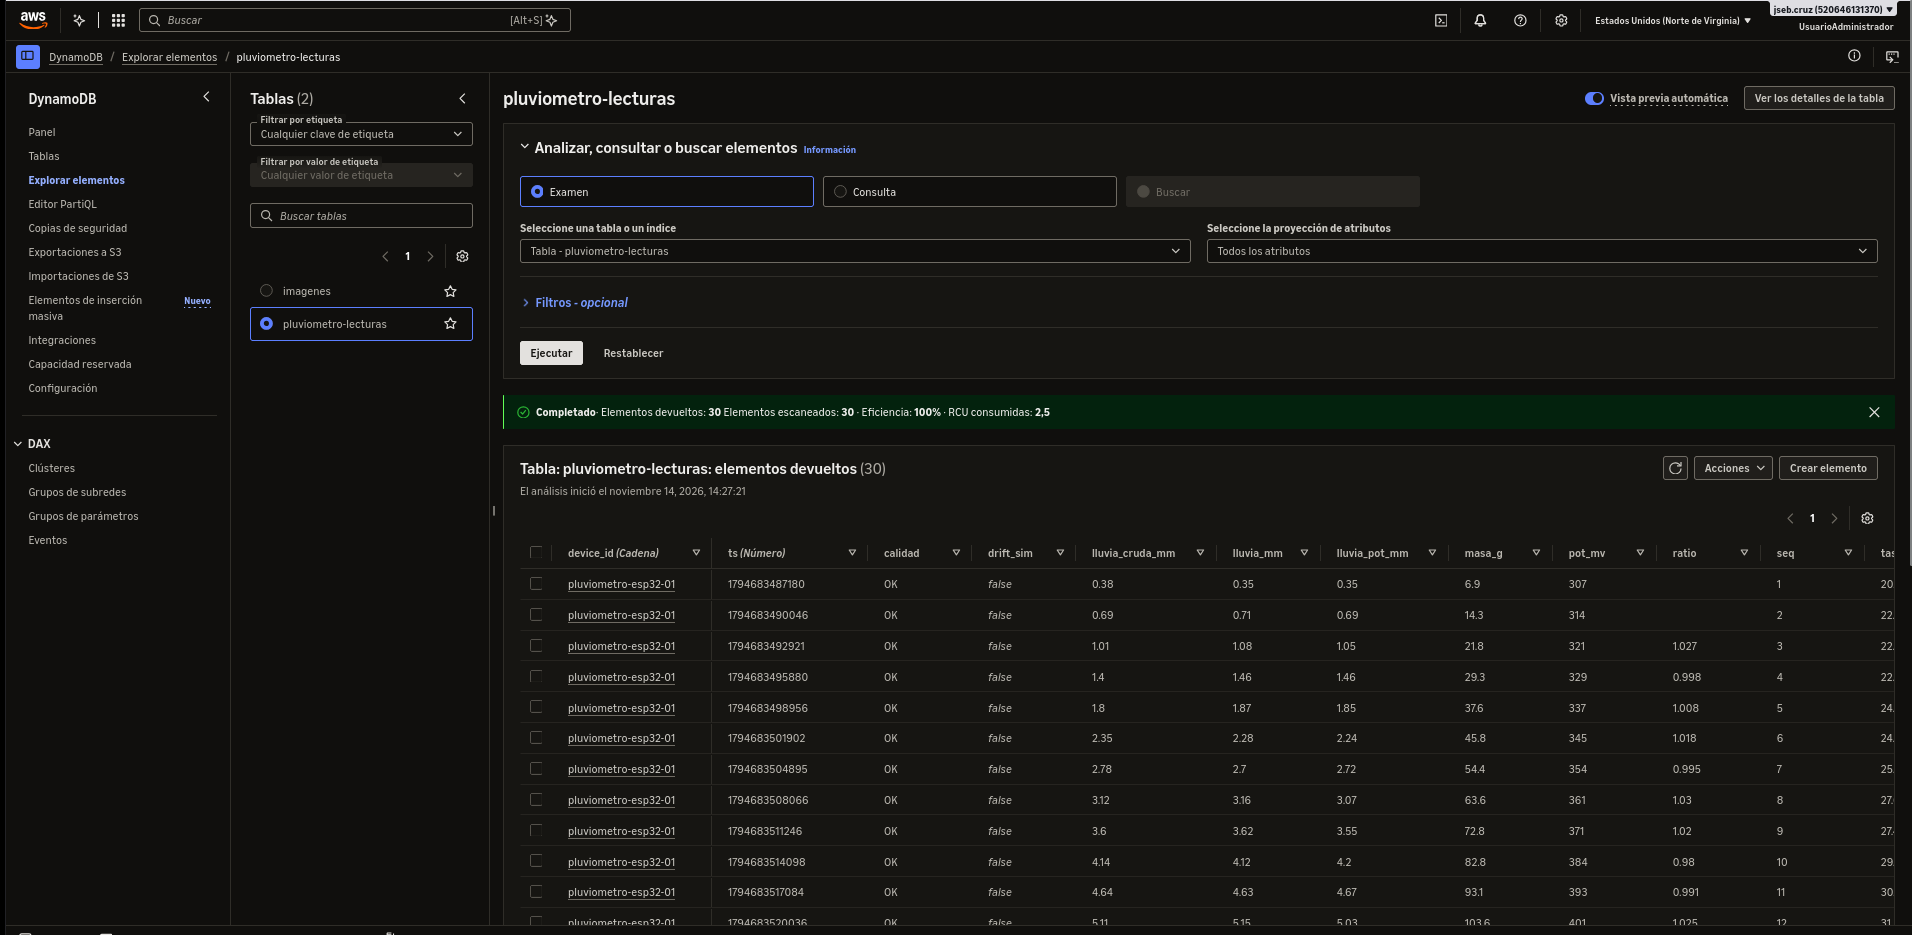
\includegraphics[width=0.95\textwidth]{../docs/evidencia/anexo_dynamodb.png}
\captionof{figure}{Consola de Amazon DynamoDB: tabla \texttt{pluviometro-lecturas} con los 30 elementos de la prueba.}
\vspace{1em}
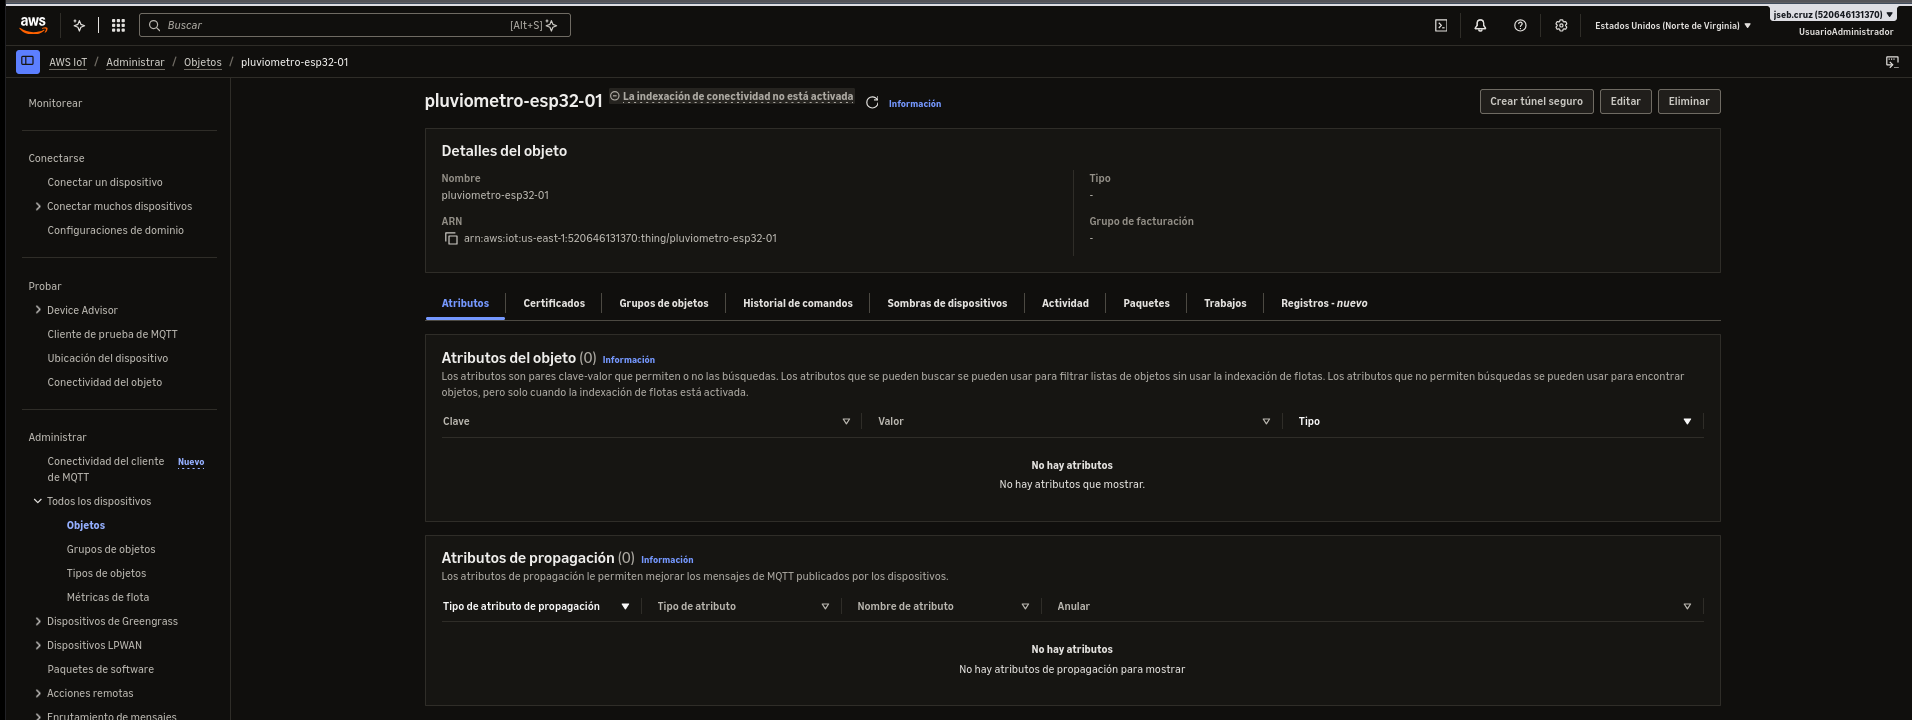
\includegraphics[width=0.95\textwidth]{../docs/evidencia/anexo_iot.png}
\captionof{figure}{Consola de AWS IoT Core: objeto \texttt{pluviometro-esp32-01} creado por Terraform.}
\end{center}

\end{document}
